An interesting constellation to study the propagation of \acp{ICME} is the so-called opposition constellation, where two planets (or other objects in the solar system) are closely aligned in heliospheric longitude. Near these oppositions, CMEs that are seen in situ at one location are most likely to be seen by the other as well, which allows to investigate their radial evolution.

In the case of Earth and Mars, whose orbital periods are 365 and 687 Earth days, respectively, an opposition occurs approximately every 780 Earth days, or 2.1 Earth years --- but this number varies slightly due to the eccentricity of Mars's orbit. Since the \textit{Curiosity} rover's landing on Mars in August 2012, such oppositions have occurred four times: In April 2014, May 2016, July 2018, and October 2020. The following study will present the first statistical study of \acp{ICME} and the associated \acp{FD} during the first two of these opposition periods. The \acp{FD}

The following article is reproduced from \textcite{Forstner-2018} with permission from Journal of Geophysical Research: Space Physics, \copyright American Geophysical Union:\\

\noindent\pubcite{Forstner-2018}\\
\strut\hfill Own contribution: 90\%

\newpage
\newcounter{includepdfpageJGREighteen}

\addtocounter{subsection}{1}
\setcounter{subsubsection}{1} 
\phantomsection
\addcontentsline{toc}{subsection}{\arabic{chapter}.\arabic{section}.\arabic{subsection} Using Forbush Decreases to Derive the Transit Time of ICMEs Propagating from 1 AU to Mars (Publication JGR--Space Physics 2018)}
%
\phantomsection
\addcontentsline{toc}{subsubsection}{\arabic{chapter}.\arabic{section}.\arabic{subsection}.\arabic{subsubsection} Introduction}
\label{sec:paper_forstner2018}
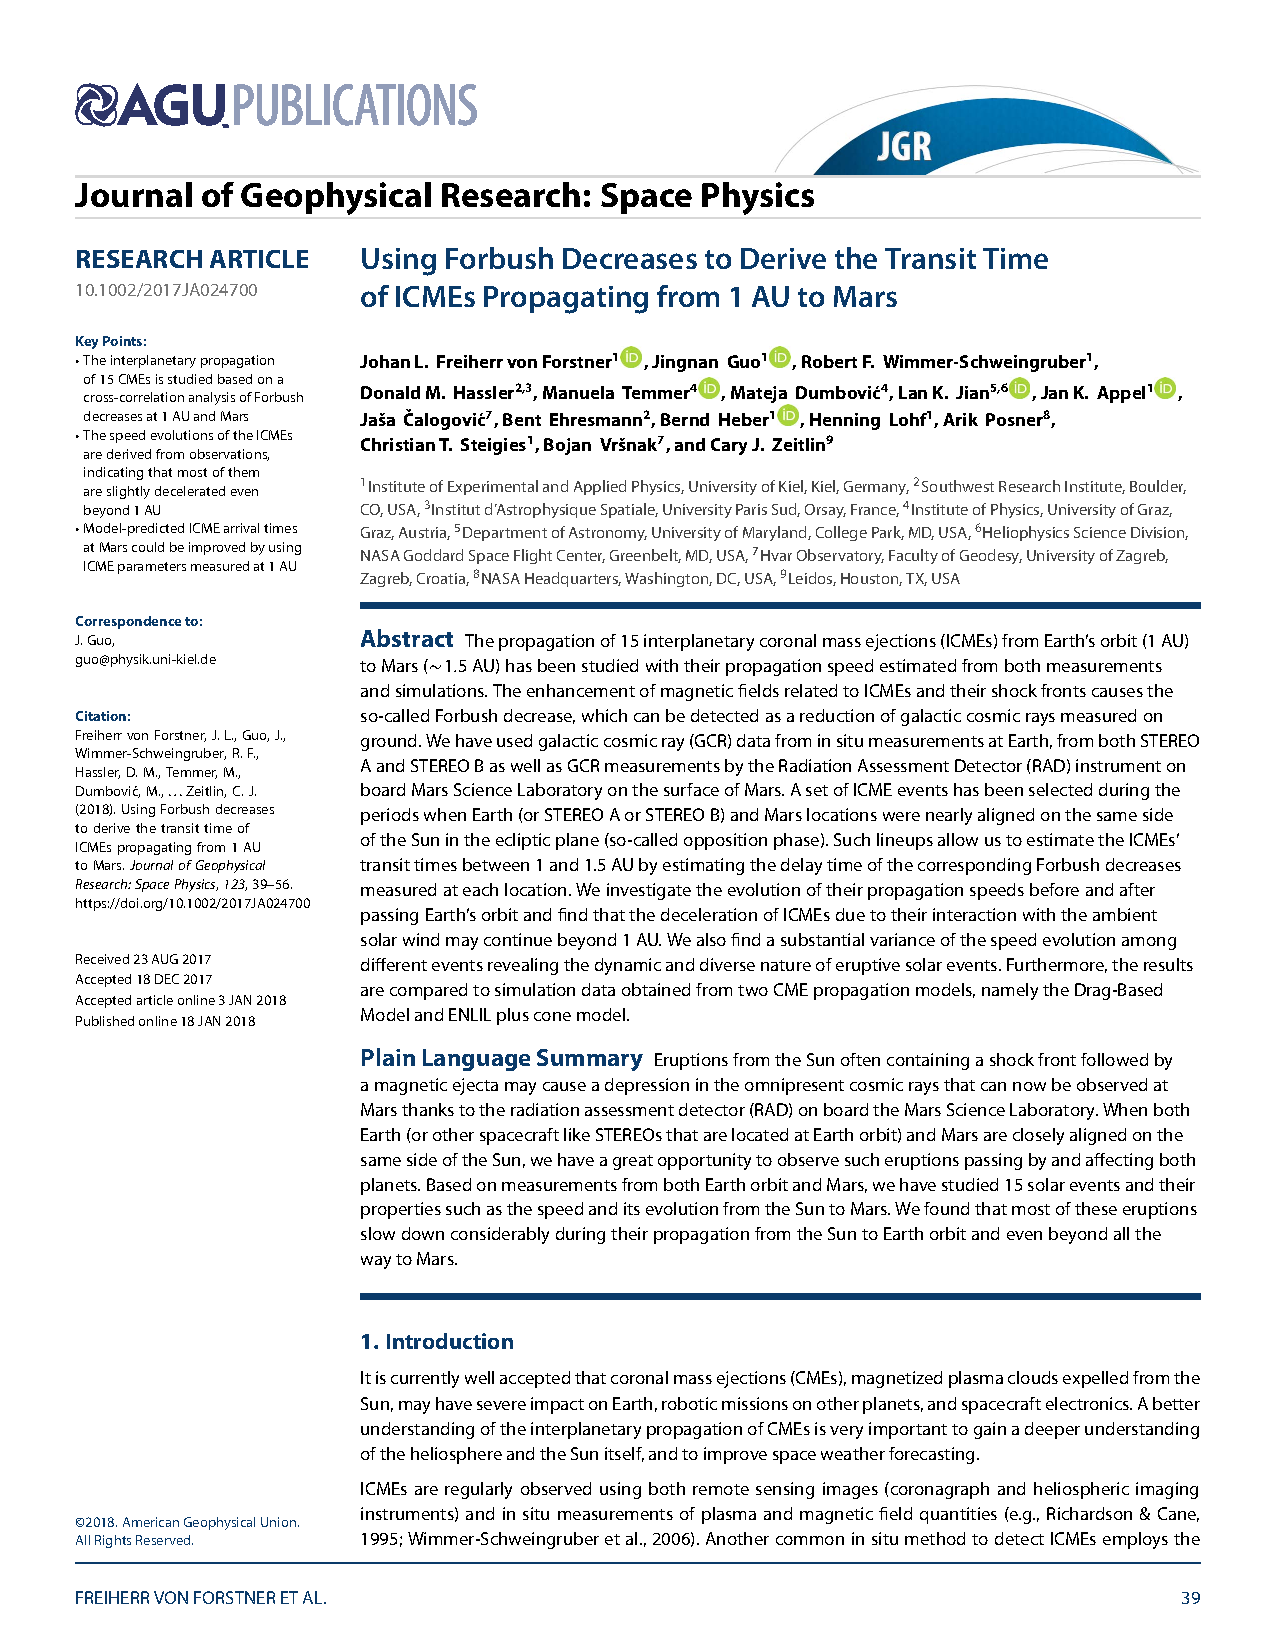
\includepdf[pages={1-2}, link, linkname=paper_forstner2018, scale=.9, pagecommand={\refstepcounter{includepdfpageJGREighteen}\label{paper_forstner2018.\theincludepdfpageJGREighteen}}]{publications/Forstner_et_al-2018-JGRSpace.pdf}
%
\addtocounter{subsubsection}{1} 
\phantomsection
\addcontentsline{toc}{subsubsection}{\arabic{chapter}.\arabic{section}.\arabic{subsection}.\arabic{subsubsection} Methods and Data}
\includepdf[pages={3-5}, link, linkname=paper_forstner2018, scale=.9, pagecommand={\refstepcounter{includepdfpageJGREighteen}\label{paper_forstner2018.\theincludepdfpageJGREighteen}}]{publications/Forstner_et_al-2018-JGRSpace.pdf}
%
\addtocounter{subsubsection}{1} 
\phantomsection
\addcontentsline{toc}{subsubsection}{\arabic{chapter}.\arabic{section}.\arabic{subsection}.\arabic{subsubsection} Results and Discussion}
\includepdf[pages={6-12}, link, linkname=paper_forstner2018, scale=.9, pagecommand={\refstepcounter{includepdfpageJGREighteen}\label{paper_forstner2018.\theincludepdfpageJGREighteen}}]{publications/Forstner_et_al-2018-JGRSpace.pdf}
%
\addtocounter{subsubsection}{1} 
\phantomsection
\addcontentsline{toc}{subsubsection}{\arabic{chapter}.\arabic{section}.\arabic{subsection}.\arabic{subsubsection} Conclusion}
\includepdf[pages={13}, link, linkname=paper_forstner2018, scale=.9, pagecommand={\refstepcounter{includepdfpageJGREighteen}\label{paper_forstner2018.\theincludepdfpageJGREighteen}}]{publications/Forstner_et_al-2018-JGRSpace.pdf}
%
\addtocounter{subsubsection}{1} 
\phantomsection
\addcontentsline{toc}{subsubsection}{\arabic{chapter}.\arabic{section}.\arabic{subsection}.\arabic{subsubsection} Appendix A: Cross-Correlation Analysis Plots for Each Event}
\includepdf[pages={14-16}, link, linkname=paper_forstner2018, scale=.9, pagecommand={\refstepcounter{includepdfpageJGREighteen}\label{paper_forstner2018.\theincludepdfpageJGREighteen}}]{publications/Forstner_et_al-2018-JGRSpace.pdf}
%
\addtocounter{subsubsection}{1} 
\phantomsection
\addcontentsline{toc}{subsubsection}{\arabic{chapter}.\arabic{section}.\arabic{subsection}.\arabic{subsubsection} References}
\includepdf[pages={17-18}, link, linkname=paper_forstner2018, scale=.9, pagecommand={\refstepcounter{includepdfpageJGREighteen}\label{paper_forstner2018.\theincludepdfpageJGREighteen}}]{publications/Forstner_et_al-2018-JGRSpace.pdf}

... wie viele weitere Events sind inzwischen im HELCATS-Katalog, die richtung Mars gingen? + blabla...`


The following article is reproduced from \textcite{Forstner-2019} with permission from Space 
Weather, \copyright American Geophysical Union:\\

\noindent\pubcite{Forstner-2019}\\
\strut\hfill Own contribution: 90\%

\newpage
\newcounter{includepdfpageSWNineteen}

\addtocounter{subsection}{1}
\setcounter{subsubsection}{1} 
\phantomsection
\addcontentsline{toc}{subsection}{\arabic{chapter}.\arabic{section}.\arabic{subsection} Tracking and Validating ICMEs Propagating Toward Mars Using STEREO Heliospheric Imagers Combined With Forbush Decreases Detected by MSL/RAD (Publication Space Weather 2019)}
%
\phantomsection
\addcontentsline{toc}{subsubsection}{\arabic{chapter}.\arabic{section}.\arabic{subsection}.\arabic{subsubsection} Introduction}
\label{sec:paper_forstner2019}
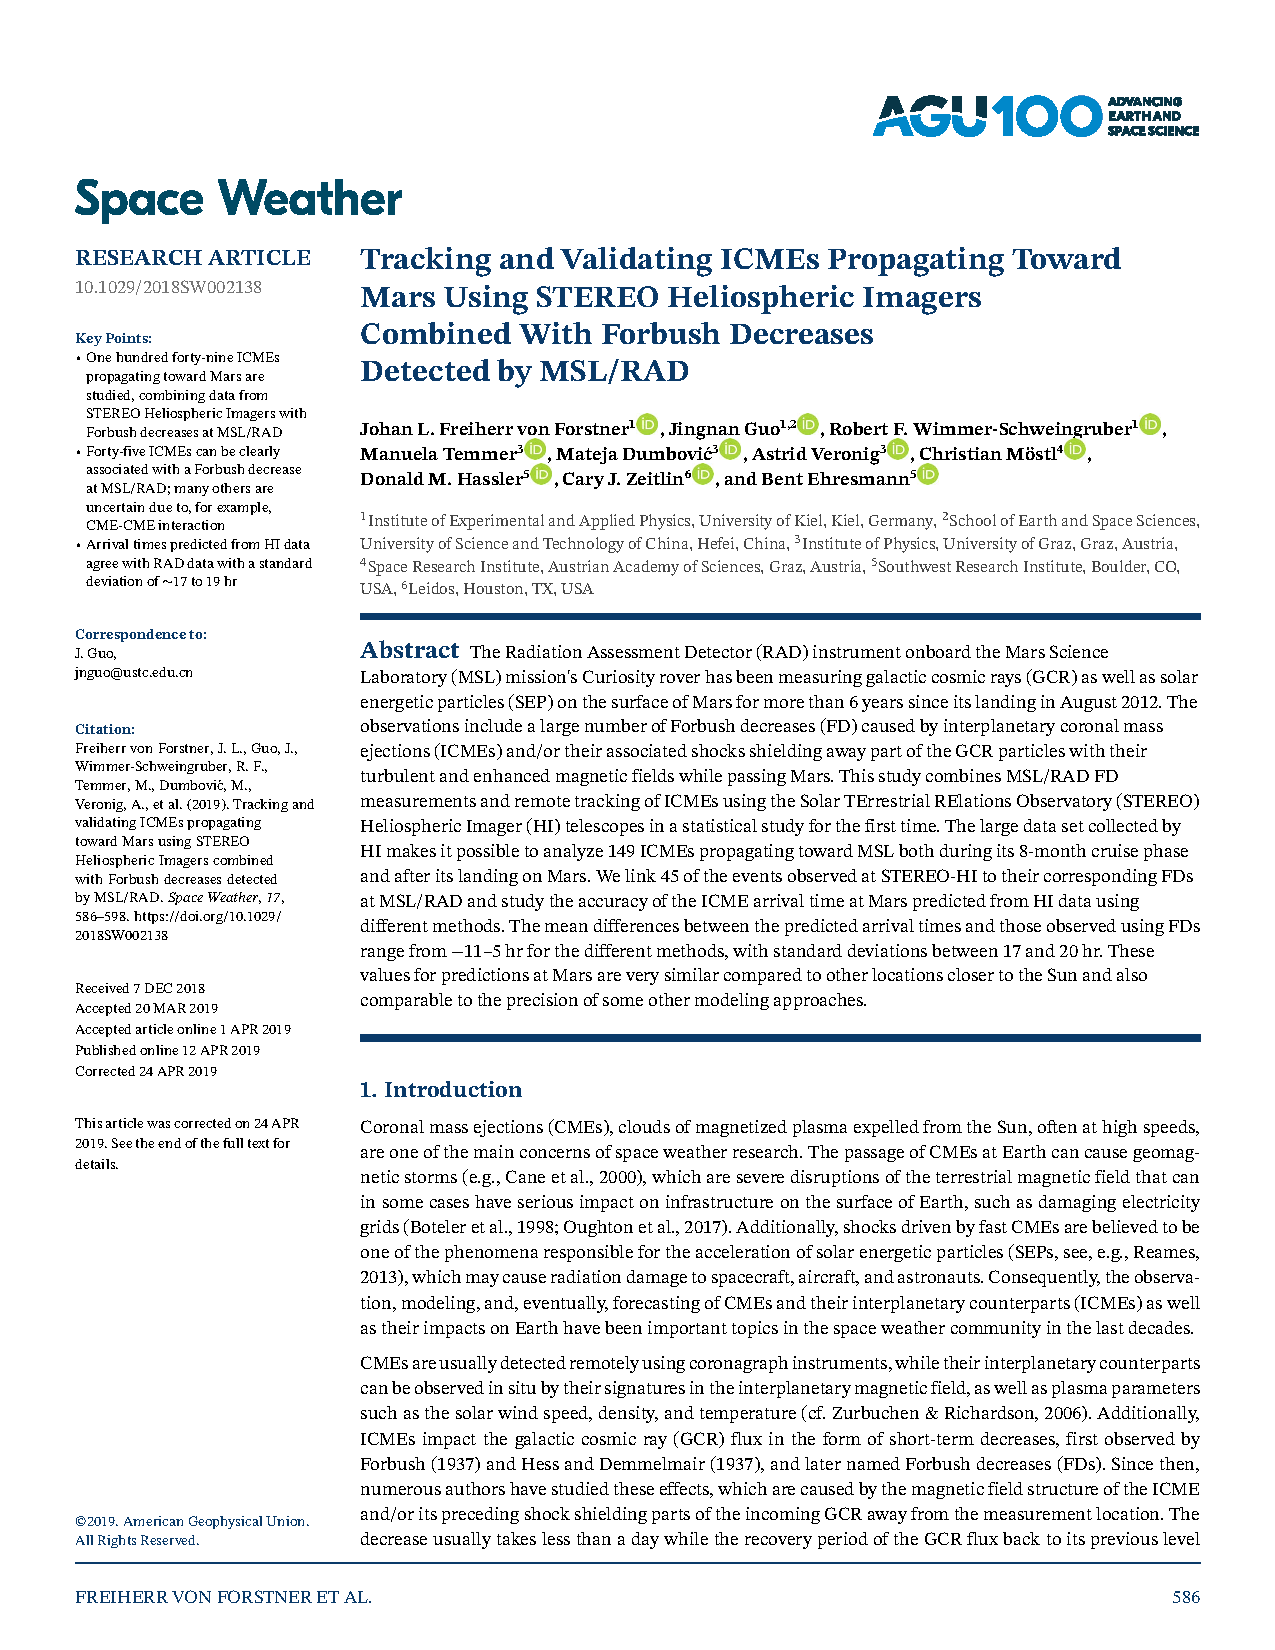
\includepdf[pages={1}, link, linkname=paper_forstner2019, scale=.95, pagecommand={\refstepcounter{includepdfpageSWNineteen}\label{paper_forstner2019.\theincludepdfpageSWNineteen}}]{publications/Forstner_et_al-2019-Space_Weather.pdf}
%
\addtocounter{subsubsection}{1} 
\phantomsection
\addcontentsline{toc}{subsubsection}{\arabic{chapter}.\arabic{section}.\arabic{subsection}.\arabic{subsubsection} Data and Methods}
\includepdf[pages={2-3}, link, linkname=paper_forstner2019, scale=.95, pagecommand={\refstepcounter{includepdfpageSWNineteen}\label{paper_forstner2019.\theincludepdfpageSWNineteen}}]{publications/Forstner_et_al-2019-Space_Weather.pdf}
%
\addtocounter{subsubsection}{1} 
\phantomsection
\addcontentsline{toc}{subsubsection}{\arabic{chapter}.\arabic{section}.\arabic{subsection}.\arabic{subsubsection} Results and Discussion}
\includepdf[pages={4-9}, link, linkname=paper_forstner2019, scale=.95, pagecommand={\refstepcounter{includepdfpageSWNineteen}\label{paper_forstner2019.\theincludepdfpageSWNineteen}}]{publications/Forstner_et_al-2019-Space_Weather.pdf}
%
\addtocounter{subsubsection}{1} 
\phantomsection
\addcontentsline{toc}{subsubsection}{\arabic{chapter}.\arabic{section}.\arabic{subsection}.\arabic{subsubsection} Conclusions and Outlook}
\includepdf[pages={10}, link, linkname=paper_forstner2019, scale=.95, pagecommand={\refstepcounter{includepdfpageSWNineteen}\label{paper_forstner2019.\theincludepdfpageSWNineteen}}]{publications/Forstner_et_al-2019-Space_Weather.pdf}
%
\addtocounter{subsubsection}{1} 
\phantomsection
\addcontentsline{toc}{subsubsection}{\arabic{chapter}.\arabic{section}.\arabic{subsection}.\arabic{subsubsection} References}
\includepdf[pages={11-13}, link, linkname=paper_forstner2019, scale=.95, pagecommand={\refstepcounter{includepdfpageSWNineteen}\label{paper_forstner2019.\theincludepdfpageSWNineteen}}]{publications/Forstner_et_al-2019-Space_Weather.pdf}

\section{Outlook}